\documentclass[tikz,border=3.14mm]{standalone}

\begin{document}

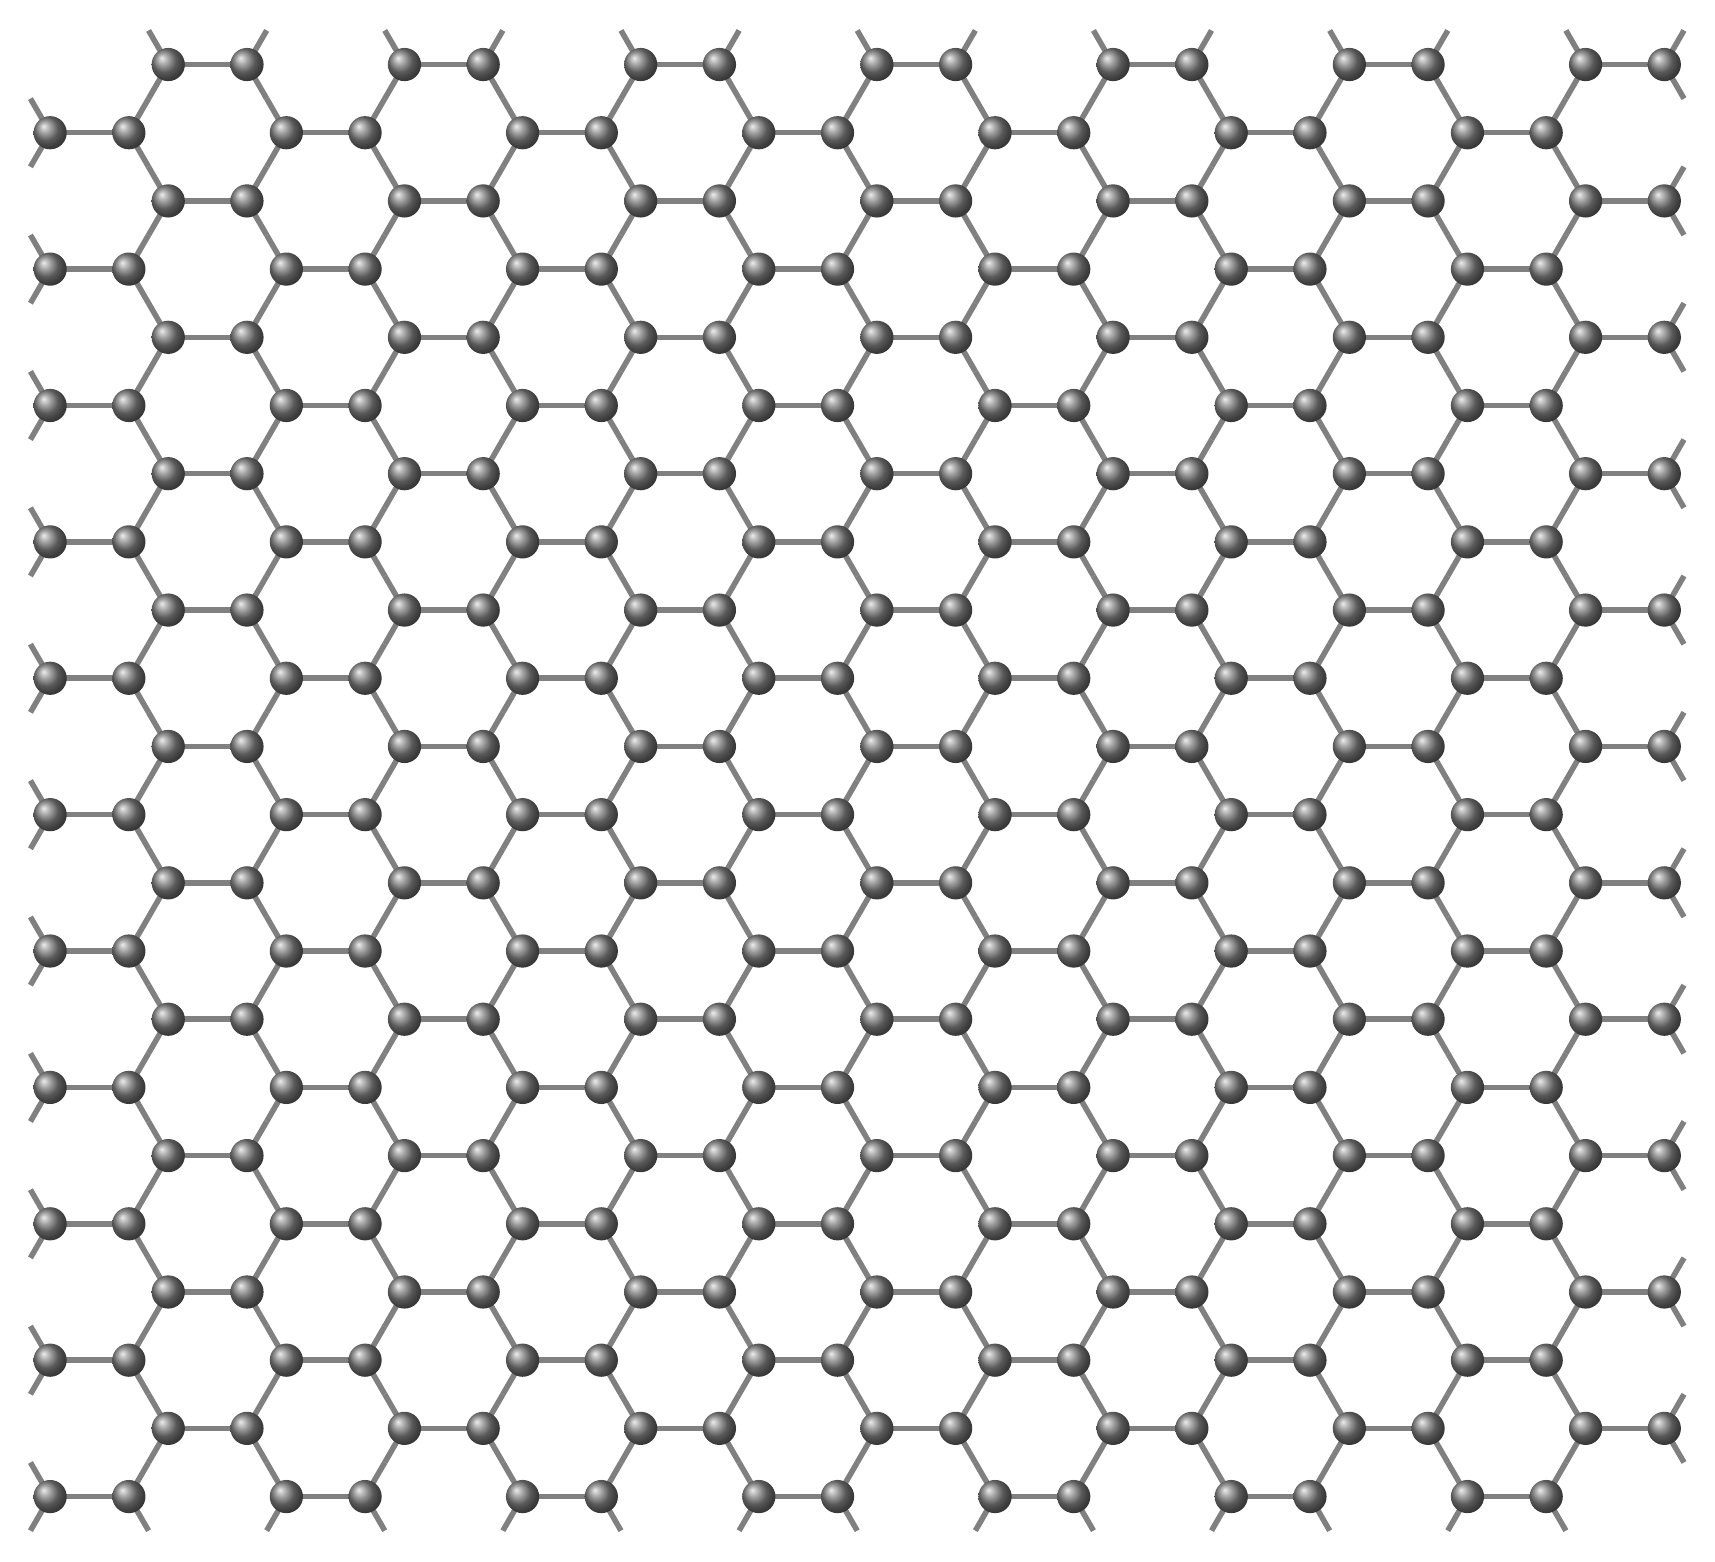
\begin{tikzpicture}[scale=1,background rectangle/.style=
{top color=black, bottom color = black}]
\def\a{1.0cm}
\def\N{6}

\def\Nx{6}
\def\Ny{10}

\begin{scope}[rotate around={0:(0,0)}]

\foreach \x in {0,1,...,\Nx}
{
    \foreach \y in {0,1,...,\Ny}
    {
        \draw[color = gray, line width=2pt] (3*\x*\a,{-\y*sqrt(3)*\a}) -- +(-{\a/4},{sqrt(3)*\a/4});
        \draw[color = gray, line width=2pt] (3*\x*\a,{-\y*sqrt(3)*\a}) -- +(-{\a/4},-{sqrt(3)*\a/4});
        \draw[color = gray, line width=2pt] (3*\x*\a,{-\y*sqrt(3)*\a}) -- +({\a/2},0);
        
        \draw[color = gray, line width=2pt] (3*\x*\a+\a,{-\y*sqrt(3)*\a}) -- +({\a/4},{sqrt(3)*\a/4});
        \draw[color = gray, line width=2pt] (3*\x*\a+\a,{-\y*sqrt(3)*\a}) -- +({\a/4},-{sqrt(3)*\a/4});
        \draw[color = gray, line width=2pt] (3*\x*\a+\a,{-\y*sqrt(3)*\a}) -- +(-{\a/2},0);
    
        \shade[ball color=gray] (3*\x*\a,{-\y*sqrt(3)*\a}) circle [radius=6pt];
        \shade[ball color=gray] (\a+3*\x*\a,{-\y*sqrt(3)*\a}) circle [radius=6pt];
    }
}

%repeat the same but with a shift

\begin{scope}[xshift=1.5*\a,yshift={\a*sqrt(3)/2}]
\foreach \x in {0,1,...,\Nx}
{
    \foreach \y in {0,1,...,\Ny}
    {    
        \draw[color = gray, line width=2pt] (3*\x*\a,{-\y*sqrt(3)*\a}) -- +(-{\a/4},{sqrt(3)*\a/4});
        \draw[color = gray, line width=2pt] (3*\x*\a,{-\y*sqrt(3)*\a}) -- +(-{\a/4},-{sqrt(3)*\a/4});
        \draw[color = gray, line width=2pt] (3*\x*\a,{-\y*sqrt(3)*\a}) -- +({\a/2},0);
        
        \draw[color = gray, line width=2pt] (3*\x*\a+\a,{-\y*sqrt(3)*\a}) -- +({\a/4},{sqrt(3)*\a/4});
        \draw[color = gray, line width=2pt] (3*\x*\a+\a,{-\y*sqrt(3)*\a}) -- +({\a/4},-{sqrt(3)*\a/4});
        \draw[color = gray, line width=2pt] (3*\x*\a+\a,{-\y*sqrt(3)*\a}) -- +(-{\a/2},0);
    
        \shade[ball color=gray] (3*\x*\a,{-\y*sqrt(3)*\a}) circle [radius=6pt];
        \shade[ball color=gray] (\a+3*\x*\a,{-\y*sqrt(3)*\a}) circle [radius=6pt];
    }
}
\end{scope}
    
\end{scope}

\end{tikzpicture}
\end{document}